% !TEX TS-program = pdflatex
% !TEX encoding = UTF-8 Unicode

% This is a simple template for a LaTeX document using the "article" class.
% See "book", "report", "letter" for other types of document.

\documentclass[12pt]{book} % use larger type; default would be 10pt

\usepackage[utf8]{inputenc} % set input encoding (not needed with XeLaTeX)

%%% Examples of Article customizations
% These packages are optional, depending whether you want the features they provide.
% See the LaTeX Companion or other references for full information.

%%% PAGE DIMENSIONS
\usepackage[right=2cm,left=3cm,top=2cm,bottom=2cm,headsep=0cm,footskip=0.5cm]{geometry}
\usepackage{geometry} % to change the page dimensions
\geometry{a4paper} % or letterpaper (US) or a5paper or....
% \geometry{margin=2in} % for example, change the margins to 2 inches all round
% \geometry{landscape} % set up the page for landscape
%   read geometry.pdf for detailed page layout information

\usepackage{graphicx} % support the \includegraphics command and options

% \usepackage[parfill]{parskip} % Activate to begin paragraphs with an empty line rather than an indent

%%% PACKAGES
\usepackage{booktabs} % for much better looking tables
\usepackage{array} % for better arrays (eg matrices) in maths
%\usepackage{paralist} % very flexible & customisable lists (eg. enumerate/itemize, etc.)
\usepackage{verbatim} % adds environment for commenting out blocks of text & for better verbatim
\usepackage{subfig} % make it possible to include more than one captioned figure/table in a single float
% These packages are all incorporated in the memoir class to one degree or another...

%%% HEADERS & FOOTERS
\usepackage{fancyhdr} % This should be set AFTER setting up the page geometry
\pagestyle{fancy} % options: empty , plain , fancy
\renewcommand{\headrulewidth}{0pt} % customise the layout...
\lhead{}\chead{}\rhead{}
\lfoot{}\cfoot{\thepage}\rfoot{}

%%% SECTION TITLE APPEARANCE
\usepackage{sectsty}
\allsectionsfont{\sffamily\mdseries\upshape} % (See the fntguide.pdf for font help)
% (This matches ConTeXt defaults)

%%% ToC (table of contents) APPEARANCE
\usepackage[nottoc,notlof,notlot]{tocbibind} % Put the bibliography in the ToC
\usepackage[titles,subfigure]{tocloft} % Alter the style of the Table of Contents
\renewcommand{\cftsecfont}{\rmfamily\mdseries\upshape}
\renewcommand{\cftsecpagefont}{\rmfamily\mdseries\upshape} % No bold!

%%% Definiendo nuevos COLORES
\usepackage{xcolor} %Paquete de Color 
\definecolor{verde}{rgb}{0.25,0.5,0.35}
\definecolor{jpurple}{rgb}{0.5,0,0.35}

%%% Configurando el Layout para mostrar codigos Java
\usepackage{listings}
\lstset{
  language=Java,
  basicstyle=\ttfamily\small,
  keywordstyle=\color{jpurple}\bfseries,
  stringstyle=\color{red},
  commentstyle=\color{verde},
  morecomment=[s][\color{blue}]{/**}{*/},
  extendedchars=true,
  showspaces=false,
  showstringspaces=false,
  numbers=left,
  numberstyle=\tiny,
  breaklines=true,
  backgroundcolor=\color{cyan!10},
  breakautoindent=true,
  captionpos=b,
  xleftmargin=0pt,
  tabsize=3
}

%%% END Article customizations

\usepackage[spanish]{babel}
\usepackage{listings} 
\newcommand{\HRule}{\rule{\linewidth}{0.5mm}}
%%% The "real" document content comes below...


\title{Investigación del Lenguaje - Java}
\author{Adriana Rodríguez \and Marcelo Sánchez \and Raquel Villón Ramíez}

%\date{} % Activate to display a given date or no date (if empty),
         % otherwise the current date is printed 


\usepackage{eso-pic}
\newcommand\BackgroundEspol{
	\put(-218,338){
	\parbox[b][\paperheight]{\paperwidth}{%
           	\vfill
	           \centering
           	
\includegraphics[height=0.07\textheight,width=0.3\textwidth,keepaspectratio]{logoespol.jpg}%
	            \vfill
}}}

\newcommand\BackgroundFiec{
	\put(245,338){
	\parbox[b][\paperheight]{\paperwidth}{%
           	\vfill
	           \centering
           	
\includegraphics[height=0.07\textheight,width=0.22\textwidth,keepaspectratio]{logofiec.jpg}%
	            \vfill
}}}


\begin{document}


\begin{titlepage}
%\hspace*{0.2in}
\AddToShipoutPicture*{\BackgroundEspol}
\AddToShipoutPicture*{\BackgroundFiec}
%
\includegraphics[height=0.1\textheight]{logoespol}
%\hspace*{2.0in}
%
\includegraphics[width=0.3\textwidth]{logofiec}
%\includegraphics[width=0.1\textwidth]
\begin{center}
\textsc{\Large Escuela Superior Politécnica del Litoral}\\[1.0cm]
\textsc{\Large Facultad de Ingenieria en Electricidad y Computación}\\[1.5cm]

% Titulo
\HRule \\[0.4cm]
{ \LARGE \bfseries Investigación de Lenguajes - JAVA \\[0.4cm] }
\HRule \\[1.5cm]


% Autores
\begin{minipage}{0.4\textwidth}
\begin{flushleft} \large
\emph{Autores:}\\
Raquel \textsc{Villón}\\
Adriana \textsc{Rodríguez}\\
Marcelo \textsc{Sánchez}
\end{flushleft}
\end{minipage}
\begin{minipage}{0.4\textwidth}
\begin{flushright} \large
\emph{Profesor:} \\
Ing.~Javier \textsc{Tibau}
\end{flushright}
\end{minipage}
\vfill
% Bottom of the page
{\large \today}
\end{center}
\end{titlepage}





%\maketitle
\tableofcontents

\newpage
\mbox{}

\chapter{Introducción}
En este primer capítulo se podrá analizar de acerca de qué es Java, conocer acerca de las principales funcionalidades así como también las características que destaca a este lenguaje orientado a objetos.

Java basicamente es un lenguaje compilador e interpretador \cite{ob} esto quiere decir que el código que genera es revisado por una máquina virtual (JVM) que lo que hace es mantener alejado el código en bytecodes sin la necesidad de revisar que sistema operativo es la que contiene la máquina en la que se está trabajando. Además, la máquina virtual ayuda con la gestión de la memoria ya que este consta con la ayuda del recolector de basura (que mantiene un control de liberación de memoria) llevan un control dinámico entre si.

El recolector de basura (\textsl{Garbage Collector}) es el encargado principal del control de la localidad de la memoria para los objetos; dicho por \cite{sun} es el responsable que los objetos estén correctamente referenciados, siendo aquellos denominados como 'vivos' mientras que los objetos que no están referenciados son considerados como objetos 'muertos' en lo que allí el recolector de basura se encarga de liberar el espacio de memoria que se había establecido para ese objeto. Un breve ejemplo sobre como ocupa espacio en la memoria tanto en llamadas como espacio se puede observar en la \textsl{Figura 1.1}.

\begin{figure}[h!]
	\begin{center}
	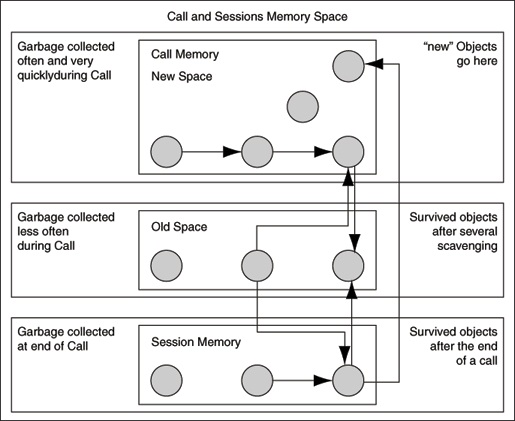
\includegraphics[scale=0.5]{garbage.jpg}
	\end{center}
	\caption{Uso del Garbage Collector en la memoria.}
\end{figure}~\\[2cm]



Se dice que Java es un OOP (Object-Oriented-Programming) \cite{oop}, contribuyendo en su sintaxis al manejo de objetos, que es un software formado a partir de un comportamiento y estado. La figura \textsl{Figura 1.2} muestra como está compuesto un objeto. \textsl{Estado} es la característica que tiene el objeto (nombre, dirección, teléfono, etc.), mientras que el \textsl{comportamiento} se refiere a la actividad que este realiza(respirar, caminar, etc.)

Otro aspecto principal con lo que está proporcionado java es por el API (Application Programmer Interface) en el posee una colección de componentes que trabajan entre si para el uso en la gestión de interfaces, redes, y en especial algoritmos que maneja encriptación y certificados. Esta información es útil principalmente para el manejo de seguirdad, cabe mencionar que el JVM también lleva crédito en el control de seguridad.

\begin{figure}[h!]
		\centering
			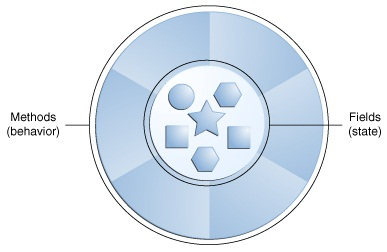
\includegraphics[width=10cm]{conceptsobject.jpg}
			\caption{A software Object.}~\\[1.4cm]
		
\end{figure}


\chapter{Características}
Entre las principales características que posee Java tenemos:

\section{Orientado a Objetos}
Mencionado anteriormente, es una de las características principales ya que por su manejo de objetos provee una mayor facilidad en la sintáxis y en el control de métodos.
\section{Robusto}
Que el lenguaje sea robusto indica que posee una mayor rigidez al momento de codificar el código, porque se va compilando para verficar que lo que se esté codificando este sin errores.
\section{Portable}
La portabilidad, ayuda en el hecho que no es necesario especificar un sistema operativo, porque consta con el JVM que hace que esta condición sea indiferente.
\section{MultiThread}
Considerado como los pocos lenguajes que maneja hilos, que son aquellos que poseen una acción específica en un periodo de tiempo. \cite{thread} indica que los hilos permiten a una aplicación ejecutar múltiples hilos parcialmente.

\chapter{Historia}
Según los hermanos Deitel (2007), el lenguaje java fue creado en 1991 por la compañía Sun Microsystems, la cual es una empresa dedicada a la fabricación y venta de servidores y componentes de componentes informáticos. Empezó como un proyecto de investigación de la compañía denominado Green y fue pensado para programar los dispositivos electrónicos inteligentes.

Deitel también indica que Java está basado en C++. Al principio su nombre fue Oak, pero luego se descubrió que ese nombre ya lo tenía otro lenguaje de programación. Luego, en una reunión de la gente de Sun en una cafetería, se propuso el nombre de Java, el cual es una variedad de café.

Al principio el proyecto Green tuvo problemas debido a que el avance de los dispositivos electrónicos inteligentes no se desarrollaba tan rápido como Sun había previsto. Sin embargo, cuando la World Wide Web explotó, Sun vio rápidamente el potencial que Java tenía para darle dinamismo a las páginas web. De esa manera el proyecto Green pudo avanzar y finalizar con una conferencia en mayo de 1995, en la que Sun Microsystems anunció formalmente la existencia del lenguaje de programación Java. 

A medida que la World Wide Web avanzaba Java tenía mayor acogida y se desarrolló de tal modo en el que luego se lo utilizó para desarrollar grandes aplicaciones empresariales, aplicaciones para dispositivos móviles, radiolocalizadores, asistentes personales digitales, entre otros. 

En el 2009, Sun Microsystems fue comprada por Oracle por un valor de 7.400 millones de dólares según el portal 20minutos.es (2009) Y actualmente se distribuye la versión número 7 de Java, así como también sus diferentes líneas. Estas líneas se especializan en un ambiente, por ejemplo: Java SE está creada especialmente para aplicaciones de escritorio; Java EE es especializado en crear aplicaciones web; Java ME es utilizado para desarrollar aplicaciones que se ejecutan en dispositivos móviles, etc.



\chapter{Tutorial de Instalación}
Para poder correr aplicaciones creadas en Java se necesita mínimo instalar Java Runtime Enviroment (JRE). Pero si lo que se quiere es desarrollar aplicaciones en Java, entonces necesita Java Development Kit (JDK) que contiene al JRE y herramientas para desarrollar, depurar y monitorear aplicaciones en Java (Oracle.com).

En este documento mostraremos la instalación  de Java SE 7, distribución para el desarrollo de aplicaciones de escritorio, en plataforma Windows 8 de 64bits. Para esto necesitaremos lo siguiente:

\begin{enumerate}
\item Descargar el JDK directamente de la página oficial de Oracle\footnote{http://www.oracle.com/technetwork/java/javase/downloads/index.html}.

\begin{figure}[!hbp]
		\centering
			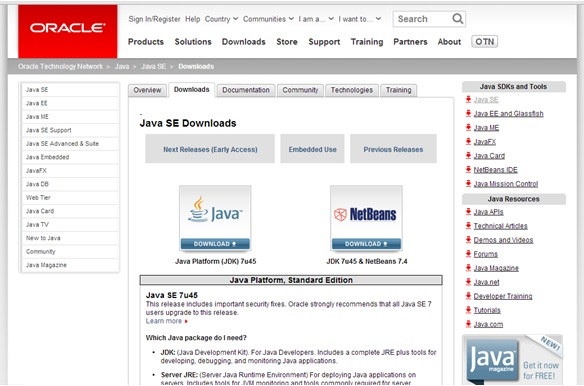
\includegraphics[width=10cm]{ins1.jpg}
			\caption{Página de descarga del JDK.}
			\label{fig1}
		
	\end{figure}
En la Figura \ref{fig1} se muestra la opción para descargar sólo el JDK o el JDK con el IDE de desarrollo creado por Oracle, NetBeans. Escogeremos descargar sólo el JDK.
	
	
	
\item Para poder descargar el JDK debemos aceptar la licencia Y escoger el instalador adecuado para el Sistema operativo que se esté utilizando como se muestra en la Figura 4.2.

	\begin{figure}[!hbp]
		\centering
			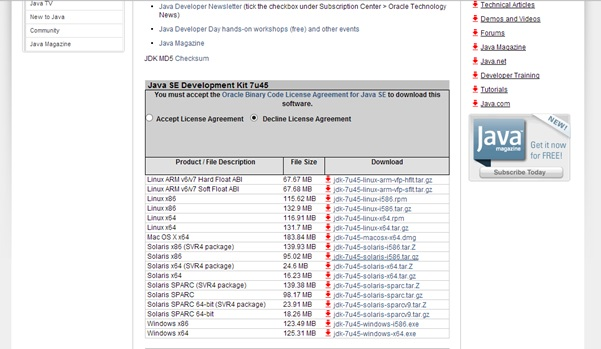
\includegraphics[width=10cm]{ins2.jpg}
			\caption{Página de descarga del JDK.}
		
	\end{figure}

\item Cuando finalice la descarga, se podrá comenzar la instalación ayudado por una wizzard de windows. de las Figuras 4.3 a 4.8

	\begin{figure}[!hbp]
		\centering
			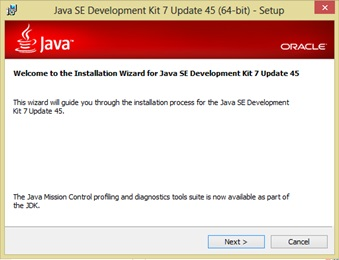
\includegraphics[width=8cm]{ins3.jpg}
			\caption{Página de descarga del JDK.}
		
	\end{figure}
	\begin{figure}[!hbp]
		\centering
			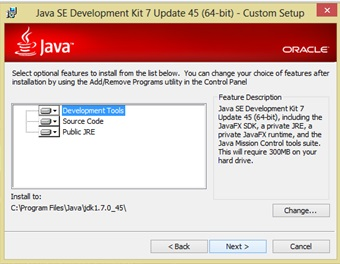
\includegraphics[width=8cm]{ins4.jpg}
			\caption{Página de descarga del JDK.}
		
	\end{figure}
	\begin{figure}[!hbp]
		\centering
			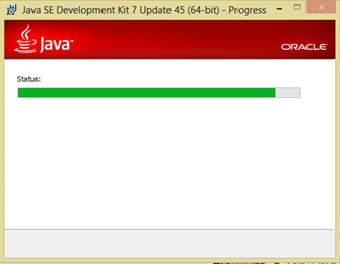
\includegraphics[width=8cm]{ins5.jpg}
			\caption{Página de descarga del JDK.}
		
	\end{figure}
	\begin{figure}[!hbp]
		\centering
			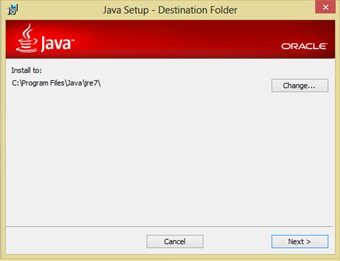
\includegraphics[width=8cm]{ins6.jpg}
			\caption{Página de descarga del JDK.}
		
	\end{figure}
	\begin{figure}[!hbp]
		\centering
			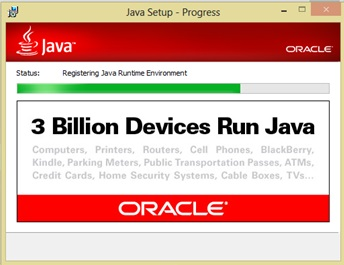
\includegraphics[width=8cm]{ins7.jpg}
			\caption{Página de descarga del JDK.}
		
	\end{figure}
	\begin{figure}[!hbp]
		\centering
			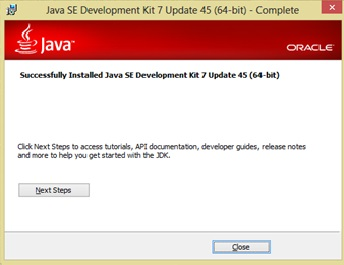
\includegraphics[width=8cm]{ins8.jpg}
			\caption{Página de descarga del JDK.}
		
	\end{figure}
	
Y listo!

\end{enumerate}

Anteriormente hubiera sido necesario agregar una nueva variable de entorno para que el sistema sepa dónde buscar el compilador y ejecutor de java. Pero desde el sistema operativo Windows 7, hacer esta especificación ya no es necesaria.


\chapter{Hola Mundo y otros Programas Introductorios}

Cada vez que se usa una computadora, esta ejecuta múltiples aplicaciones que realizan tareas para el usuario. Los programadores, son los encargados de elaborar estas aplicaciones, escribiendo programas de cómputo que permiten a los usuarios cumplir sus tareas diarias.
Ahora vamos a considerar la tarea de programar una aplicación sencilla, la cual muestra únicamente una línea de texto con el mensaje ``Hola mundo", en consola, esta aplicación sera la base para demostrar que programar en Java es fácil, todo programador ha escrito estas lineas de código, probablemente en sus inicios en este lenguaje de programación.
Para esto necesitaremos hacer uso de un IDE\footnote{Existen otros IDEs para programar en Java tales como; Netbeans, JCreator, Processing, BlueJ, Kawa, JBuilder, DrJava, entre otros disponibles en la web}, en este ejemplo usaremos el IDE de Java, Netbeans en su mas reciente version, el cual ya habremos instalado previamente. \\Para crear una aplicación en Java debemos ir al menú de Archivo y, a continuación hacer clic en Nuevo Proyecto.

En la ventana que se despliega a continuación (fig. \ref{hw01}) en el área de Categoría hacemos clic en Java y en el área de Proyecto, hacemos clic en Java Application, luego damos clic en siguiente.

	\begin{figure}[h]
		\centering
			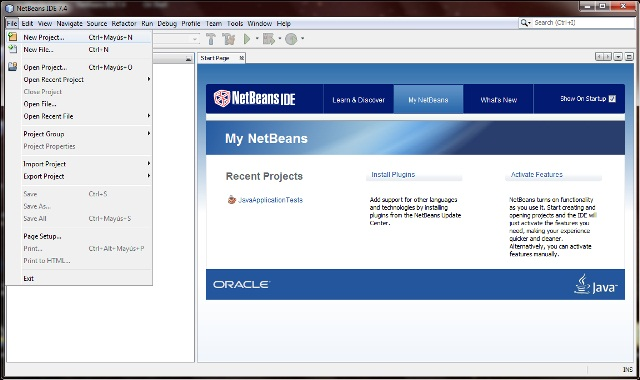
\includegraphics[width=16cm]{Hola_mundo_001.jpg}
			\caption{Ventana Principal, Netbeans.}
			\label{hw01}
	\end{figure}

En la nueva ventana(fig. \ref{hw02}), en el recuadro de Nombre del Proyecto, escribimos un nombre\footnote{El nombre no debe contener espacios en blanco ni caracteres especiales, para evitar posibles conflictos, también se recomienda que sea corto y altamente descriptivo.}, luego hacemos clic en siguiente.

	\begin{figure}[h]
		\centering
			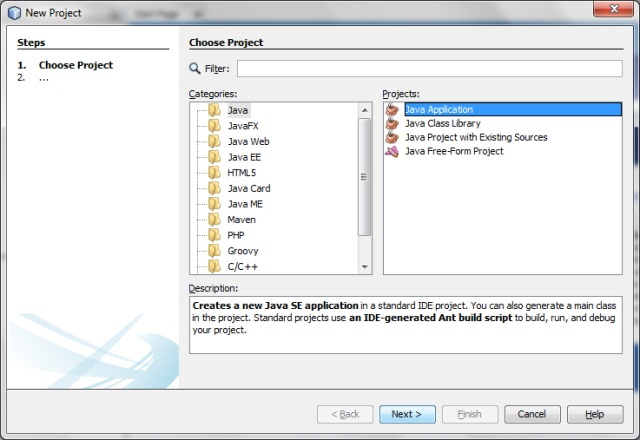
\includegraphics[width=12cm]{Hola_mundo_002.jpg}
			\caption{Ventana Nuevo Proyecto, Netbeans.}
			\label{hw02}
	\end{figure}

Ya en la ventana de nuestro nuevo proyecto(fig. \ref{hw03}), podemos notar que luego de la linea:

	\begin{figure}[h]
		\centering
			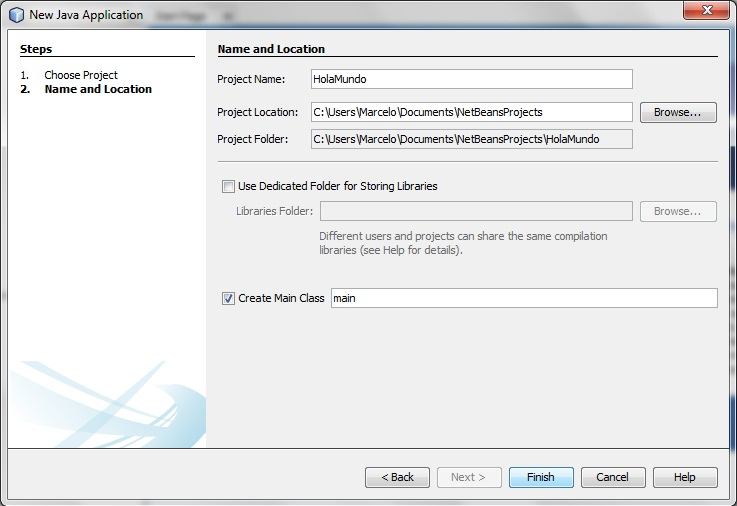
\includegraphics[width=12cm]{Hola_mundo_003.jpg}
			\caption{Ventana Nueva Aplicación Java, Netbeans.}
			\label{hw03}
	\end{figure}


\noindent
\begin{lstlisting}[frame=single]
   public static void main (String argv[])
   {
     // Todo el CODIGO va AQUI
     
   }
\end{lstlisting}

Existe un comentario que dice ``Todo el CÓDIGO va AQUÍ", y es porque es allí donde debemos escribir la función para imprimir el mensaje en pantalla, el código quedaría de la siguiente manera.

\noindent
%
\begin{lstlisting}[frame=single]
/**
 * Este es un comentario
 */
 public class HolaMundo {
   public static void main (String argv[])
   {
     // Este tambien es un Comentario
     System.out.println("Hola mundo!");
   }
 }
\end{lstlisting}

Una vez escritas las lineas de código, pulsamos la tecla F5 o en su defecto vamos al menú Ejecutar, Ejecutar Proyecto.

Y si esta todo correctamente escrito como en la fig. \ref{hw04}, en consola se debería mostrar el mensaje: Hola mundo!.

	\begin{figure}[h]
		\centering
			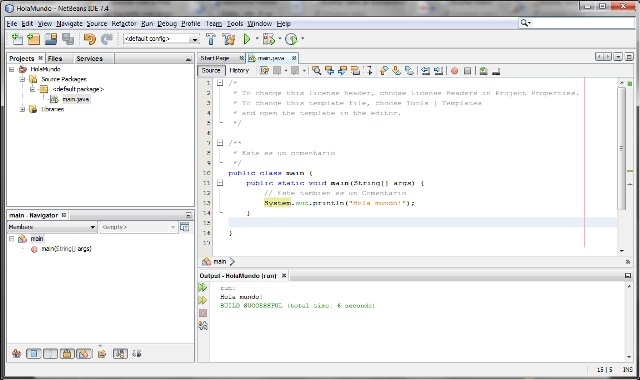
\includegraphics[width=16cm]{Hola_mundo_004.jpg}
			\caption{Ejecución correcta, Aplicación Java.}
			\label{hw04}
	\end{figure}
	
\begin{thebibliography}{99}
\bibitem{ob} Belmonte, O. (2005). \textsl{Introducción al lenguaje de programación Java}. [en línea]. Disponible en: http://www3.uji.es/belfern/pdidoc/IX26/Documentos/introJava.pdf.

\bibitem{sun} Sun Microsystems. (2006). \textsl{Memory Management in the Java Virtual Machine} [en línea]. Disponible en: http://www.oracle.com/technetwork/java/javase/memorymanagement-whitepaper-150215.pdf

\bibitem DEITEL, Paul J. y Harvey M. DEITEL (2007). \textsl{Cómo Programar en Java}. México..Pearson Education. 

\bibitem Portal 20Minutos.(2013). \textsl{Oracle compra Sun Microsystems} [en línea]. Disponible en: http://www.20minutos.es/noticia/464024/0/oracle/compra/sun/

\bibitem{oop} Sun Microsystems. \textsl{Object-Oriented Programming Concepts} [en línea]. Disponible en: http://docs.oracle.com/javase/tutorial/java/concepts/

\bibitem{thread} Oracle. \textsl{API Java-Thread} [en línea]. Disponible en: http://docs.oracle.com/javase/1.4.2/docs/api/java/lang/Thread.html

\end{thebibliography}

\end{document}
